\documentclass[10pt, oneside, a4paper]{article}

%\usepackage[colorlinks,bookmarksopen]{hyperref}

\usepackage[utf8x]{inputenc}
%\usepackage{pifont,alltt,amsmath,theorem}
\usepackage[catalan]{babel}
\usepackage{graphicx}
\usepackage{longtable}
\usepackage{fullpage}

\title{ Accessibility in Theaters using Mobile Devices \\ Project Description \& Schedule}

\author{Oscar Lopes
\\ 
Center for Ambient Intelligence and Accessibility of Catalonia
%\\ (CaiaC)
\\ Universitat Autònoma de Barcelona}
\date{\today}

\makeindex

\begin{document}

\maketitle

\section{System Description}

The main idea is to develop a message distribution system, for subtitles and audio descriptions in multi-lingual context, adapted for show rooms, providing access to both people who have sensory disabilities (visual or auditory) as for people who have difficulty understanding language in used in the show.

The system is based on a mobile device (Android, iPhone,...) with a screen to read the subtitles and a headphone output for audio description. These mobile devices are connected through a network without children, a computer system that distributes content such as multiple messages, subtitles, audio descriptions, ..., in the language you have chosen from among the spectators that offers the show. The system architecture is describded in Figure \ref{figs:systemarch}.

In a initial development phase the theaters that have shown interest in this project are:
\begin{itemize}
\item Liceu
\item Teatre Nacional de Catalunya (TNC)
\item Teatre Lliure
\end{itemize}

\begin{figure}[t]
\centering
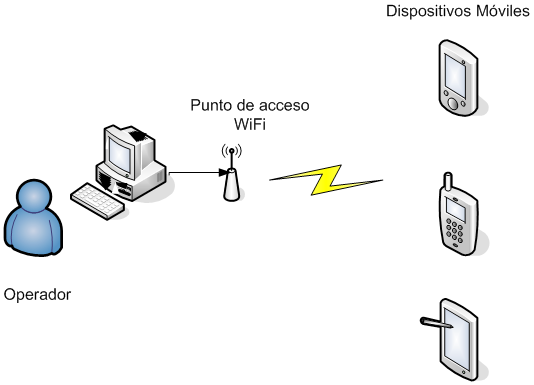
\includegraphics[scale=2.5]{pics/arch.png}
\caption{System Architecture}
\label{figs:systemarch}
\end{figure}

\section{Operation Modes}
The system is planned to have three ways of triggering the broadcast of the contents during the shows.

\begin{enumerate}
	\item \textbf{Automatic}: When the timings to launch the contents is well known .
	\item \textbf{Manual}: When is required the presence of an operator to launch the contents.
	\item \textbf{Intelligent}: The system detects a new sentence spoken by the actor, and broadcasts the corresponding content (This mode will be postponed to some later version).
\end{enumerate}

%This system is protected by patent.


\section{Users}
The system must take into account three types of users, each one requiring different functionalities:
 
\begin{description}
	\item[Administrator]: Manages the content \& configuration of the broadcasting server:
	\item[Operador]: Controls the server sessions during a show.
	\item[Spectator]: Using the mobile device, receives the contents related to the show.		
\end{description}


\section{Server Funcionalities}
Next are describded the functionalities required from the content server. There are two main user types: an Operator and an Administrator. 

\subsection{Administrator}
This user has total control of the server's functionalities and configurations. It has the following roles:
\begin{itemize}
	\item Create new users
	\item Import to the system new content (subtitles, audio descrition, etc) from the STR2 format defined by UAB.
	\item Delete from the system content that is no longer required.
	\item Configure the promotional advertisement that is broadcasted during the breaks.
\end{itemize}

\subsection{Operator}
\begin{itemize}
	\item Create a new session for broadcasting contens.
	\item Select the contens to be broadcasted during the show and the translated languages.
	\item Configure the the contents launching mode (manual, automatic, etc)
	\item Switch the between the states ''show time'' (content broadcasting) and "advertisement"
\end{itemize}

\section{Functionalities of the Mobile Device}
In this section is describded the functionalities required on the spectators's mobile device, or on the devices available on the theater.

\subsection{Espectador}
\begin{itemize}
	\item Select user interface language.
	\item Select the language of the contents broadcasted on the show.
	\item Choose the type of desired contents (subtitle, audio descriptions, etc...).
	\item Read the contents on the mobiles's device screen, in the language previouly selected.
	\item Identify the actor that is currently speaking (by color or by the actor's name) 
	\item Audio descriptions for blind people with the content pre-recorded. 
	\item In the intervals the spectator receives advertising / promotional information.
	\item Usage of the infrastructure as sound amplifier (Problem: the delay / desinchronization can be high).
\end{itemize}

\section{Non Functional Requirements}
\begin{itemize}
	\item Disable the speaker of the mobile device (to be able to hear audio it is required to plug-in headphone)
	\item Compatibility with the mobile operatinf systems: \emph{Android}, \emph{BalckBerry} and \emph{iPhone} (The first prototype will be developed in \emph{Android}).
	\item The screen of the mobile device must have a dark color, with low luminosity.
	\item The application can be downloaded from the online app store (Android Market)
\end{itemize}

\section{Liceu custom feature requests}
\begin{itemize}
	\item The client application installed on the smartphone must deactivate the mobile applications inbound events, as far as possible, and also block inbound calls and activating silence mode, etc.
	\item While the application is active it should run in full screen mode, to block access to other functionalities, not required in "show time".
	\item Make the application fault tolerant to broadcast failure, network timeouts, ...
	\item The subtitles font should dinamically adapt to the total size of the received text, so it guarantees it is shown on the mobile screen.
	\item The systems must support multiple languages: catalán, spanish and english.
	\item The systems must be compatible with the subtitling software VICOM content generator.
	\item Sound only works only the applications has the headphones plugged-in.
\end{itemize}

\newpage
\section{Feature List}

\begin{center}
	
	\begin{longtable}{ | c | p{6cm} | c | p{5cm} |}
	\hline
	Feature ID & Description & Component & Comment \\ \hline
	\hline
	\hline
	001 & The system must support multiple languages (English, Catalan, Spanish, etc) & Content Generator & \\ \hline
	002 & Include a subtitle previewer & Content Generator & \\ \hline
	003 & The contents must be exported in a single file (with subtitles, audio, etc) & Content Generator & \\ \hline
	004 & Must be compatible with VICOM subtitles system & Content Generator & VICOM is a proprietary system. Some example files must be obtained to close this task\\ \hline
	005 & Audio descriptions should be generated using Festival and/or by custom audio recorder  & Content Generator & \\ \hline
	006 & Support chain of translations. Use one subtitle translation as the original text of another. This is required since the translation probably is not made by the same translator.  & Content Generator & \\ \hline
	007 & Support Administrator and Operator(s) user roles & Server & \\ \hline
	008 & Support creation/deletion of new users & Server & \\ \hline
	009 & Administrator can import new content & Server & \\ \hline
	010 & Operator can create and control a session for content broadcasting, selecting the languages to use & Server & \\ \hline
	011 & Administrator can configure the promotional advertisement that is broadcasted during the breaks.  & Server & \\ \hline
	012 & Operator can configure the the contents launching mode (manual, automatic, etc) & Server & \\ \hline
	013 & Operator can switch the between the states ''show time'' (content broadcasting) and "advertisement" & Server & \\ \hline
	014 & Integrate the media streaming server for broadcasting of the audio to the clients & Server & \\ \hline
	015 & Select the user's interface language & Mobile Device & \\ \hline
	016 & Select the language received from the broadcast & Mobile Device &\\ \hline
	017 & Choose the type of desired contents (subtitle, audio descriptions, etc...) & Mobile Device &\\ \hline	
	018 & Read the contents on the mobiles's device screen, in the language selected & Mobile Device &\\ \hline	
	019 & Identify the actor that is currently speaking (by color or by the actor's name)  & Mobile Device &\\ \hline
	020 & Support audio descriptions for blind people with the content pre-recorded & Mobile Device &\\ \hline
	021 & Receive advertising / promotional information & Mobile Device &\\ \hline
	022 & Usage of the infrastructure as sound amplifier  & Server &\\ \hline
	023 & Usage of the infrastructure as sound amplifier  & Mobile Device &\\ \hline
	024 & Disable the speaker of the mobile device (to be able to hear audio it is required to plug-in headphone) & Mobile Device &\\ \hline
	025 & The screen of the mobile device must have a dark color, with low luminosity & Mobile Device &\\ \hline
	026 & The client application installed on the smartphone must deactivate the mobile applications inbound events, as far as possible, and also block inbound calls and activating silence mode, etc & Mobile Device &\\ \hline
	027 & While the application is active it should run in full screen mode, to block access to other functionalities, not required in "show time" & Mobile Device &\\ \hline
	028 & Sound only works only the applications has the headphones plugged-in & Mobile Device &\\ \hline
	%029 &  & &\\ \hline
	%030 &  & &\\ \hline

	\hline
	\end{longtable}

\end{center}

\end{document}


